\documentclass[11pt]{article}

\usepackage{witsa4}

\usepackage{url}
\usepackage{natbib} % Force natbib.sty to put citation labels in the reference list
\makeatletter
\renewcommand\NAT@biblabel[1]{\def\citeauthoryear##1##2{##1 ##2}[#1]\hfill}
\renewcommand\NAT@bibsetup[1]{%
  \setlength{\itemsep}{\bibsep}\setlength{\parsep}{\z@}}
\def\@lbibitem[#1]#2{%
  \if\relax\@extra@b@citeb\relax\else
    \@ifundefined{br@#2\@extra@b@citeb}{}{%
     \@namedef{br@#2}{\@nameuse{br@#2\@extra@b@citeb}}}\fi
   \@ifundefined{b@#2\@extra@b@citeb}{\def\NAT@num{}}{\NAT@parse{#2}}%
   \item[\hfil\hyper@natanchorstart{#2\@extra@b@citeb}\@biblabel{#1}%
    \hyper@natanchorend]%
    \NAT@ifcmd#1(@)(@)\@nil{#2}}
\makeatother


\bibliographystyle{named-wits}
\bibpunct{[}{]}{;}{a}{}{,}  
\usepackage{graphicx}
\usepackage{placeins}
\usepackage[nottoc,numbib]{tocbibind}
\usepackage{color}
\usepackage{xcolor}
\usepackage{listings}

\usepackage{caption}
\DeclareCaptionFont{white}{\color{white}}
\DeclareCaptionFormat{listing}{\colorbox{gray}{\parbox{\textwidth}{#1#2#3}}}
\captionsetup[lstlisting]{format=listing,labelfont=white,textfont=white}

\usepackage{titling}
\newcommand{\subtitle}[1]{%
  \posttitle{%
    \par\end{center}
    \begin{center}\large#1\end{center}
    \vskip0.5em}%
}


\title{Research Proposal:\\ Online Adaptive Content Personalisation}
\subtitle{Supervisor: Benjamin Rosman}
\author{Author: Jonathan Wasson 463117}

\begin{document}
\nocite{*}
\pagenumbering{roman} 
    
\begin{titlepage}
\maketitle
\thispagestyle{empty}
\setcounter{page}{0}

\begin{center}
    
\includegraphics[width=0.5\textwidth]{WITS-logo.jpg}
\end{center}

\clearpage



\section*{\centering{Abstract}}

Personalisation is starting to play a major role in modern software and hardware. Software that can adapt to the specific user's needs and preferences is more marketable as it has a broader range of uses. An example of this would be the current generation of computer games. Games that can provide new content to the player based on their skill level would target a larger audience, by targeting challenging game-play to skilled players and alternatively content which will not be frustratingly difficult to new or unskilled players. Content could also scale to match the player's enjoyment such that they remain engaged for as long as possible, perhaps through increasing difficulty which scales appropriately. 

\vspace{6.0 mm}

For example, a game such as `Temple Run' (which is a popular game on smart-phones) may be able to infer the user's ability and then adapt the games overall difficulty accordingly. Perhaps even infer the user's current enjoyment in the game and actively provide different content, such as unique goals or events, to maintain the user's enjoyment.

\vspace{6.0 mm}

This research proposal proposes an experiment which will involve human users playing a game that uses an adaptive algorithm to optimize the user experience and enjoyment. The results of the experiment will provide insight into the usage of an adaptive algorithm which generates content in real-time (online).


\clearpage

\tableofcontents

\end{titlepage}
\clearpage
\pagenumbering{arabic} 
\section{Introduction}
As computers begin to encroach on every aspect of everyday life, it has become more and more apparent that the diversity of people using computers is also increasing. This dependence on technology permeates most modern businesses and households. From doctors to store clerks, most will have to make use of a computer at some point in their everyday lives \citep{beaudry2005understanding}. Take doctors for example; Doctors must make use of software that can keep track of patient records as well as machinery that performs complicated procedures on patients. New technology has been developed that allows surgeons to operate over long distances through the use of the internet and augmented reality, allowing countries without the necessary skilled labour to import it from overseas almost instantaneously in cases of emergency.
\vspace{6.0 mm}

However, this progress has left a few behind. Older people, the disabled and often those who are not technologically savvy are struggling to adapt to the rigours of modern life. Nowadays, we can see old people who would have once refused to use things such as email or phones are now being forced to use these services and devices on a daily basis. Disabled people  are also being forced to adapt to this change since most devices are designed in a way that is not suitable for their use\citep{gajos2008improving}. Indeed, this ever increasing reliance on technology has forced people to adapt to modern times and it can be said that the modern worker must be able to use a computer or face the risk of unemployment.
\vspace{6.0 mm}

The research described in this document will focus on content adaptation in computer games performed in real-time. As was said previously, content adaptation has a wide variety of uses but we have decided to use it in computer games. This was done due to the relative ease at which an experiment could be created and conducted in conjunction with a computer game. There are a wide variety of computer games that can be picked from which will give us room to mould the game into something that will yield better results with little room for confusion. In performing this research it is necessary to provide examples of where the research can be implemented, which there is an abundance of. In doing this we will show the impact and commercial aspect of this research as a whole.
\vspace{6.0 mm}

To justify this as a research topic we must analyse all available media that provides insight into this topic. The following paper will discuss material relevant to this question and then use it to justify this as a research topic. We will begin by reviewing relevant research that has been conducted in the field of content adaptation and then tying this in to what we aim to achieve. Following this, we will lay out the experiment we shall be performing and the results that we hope to achieve with said experiment. Then in conclusion we will discuss the overall impact of the expected results and any work that could follow.
\vspace{6.0 mm}

The rest of this document is structured as follows: Chapter 2 will provide an overview of related work and its relevance to the work we aim to achieve. Section 2.2 provides the significance of the problem. Section 2.3 will give the reader an understanding of Markov Decision Processes and how this relates to the problem. Chapter 3 describes how the research will be done with section 3.2 providing the motivation for the choice in method. Section 3.3 is broken up into several smaller subsections, each explaining a step in the research process. Reasons and explanations will be given through out this chapter as to why each step of the experiment is conducted. Chapter 4 will then go on to explain what results we expect to obtain from this research, why this is relevant and hopefully what future work can be done in this field. Finally, chapter 5 concludes the proposal with a summary and a brief overview of the research.



\clearpage

\section{Background and Related Work}
\subsection{Introduction}
This chapter's first aim is to provide an insight into the work (as well as the works viability) which has been done in creating adaptive content. It is motivated by the need for future pieces of software to appeal to a wider audience as well as to provide this audience with a more personal and enjoyable experience.
\vspace{7.0 mm}

Currently there are several computer games that provide adaptive content to its user base. However, these implementations are not very intricate. With most implementations requiring a calibration phase (i.e. the decision of the content is decided upon by direct input). Very few games actually using a real machine learning algorithm to determine the best content to present the user with. Thus, the second aim of this section is to expound upon and to improve current methods being used to generate adaptive content. Therefore this chapter will discuss in detail the viability of this research by scrutinizing relevant and related works.
\vspace{7.0 mm}

\subsection{Significance}
\subsubsection{Uses of Adaptive Content}

As technology has improved, hardware is now capable of handling adaptive content. Previously, adaptive content has not been used as the hardware could not handle the extra computation required to adapt content in real-time and there were not many methods available to developers to successfully create adaptive content.
\vspace{7.0 mm}

The uses of adaptive content are many. In almost any software field, adaptive content could be implemented to improve the software. To fully explain just how broad and monumental adaptive could be in the computing world, I'll provide some examples below of where it could be implemented and where it has been implemented in lesser ways.

\vspace{4.0 mm}
\textbf{Gaming}
\vspace{4.0 mm}

Most games nowadays try appeal to a larger audience. This is done so that computer game companies can sell more copies of their games and in doing so make more money. There is a downside to this though, adaptive content means more content has to be created. Since more content has to be created, some of which each player might not even use, more money and development time must be spent in creating this content. The methods to implement such content is not up to scratch either.
\vspace{7.0 mm}

Games such as MMORPGs (Massively Multiplayer Online Role-Playing Games) are already starting to push out adaptive content. Most MMORPGs have monthly subscription fees as well as being story driven. The audience of these games expect to be able to make decisions that affect the outcome of the games storyline. This means that developers have to make multiple endings and storylines from which the player can pick from. Certain games, such as the Mass Effect \textsuperscript{TM} series( Trademark of the Bioware company), tackled this problem by creating large trees representing decisions which the player the `traversed' along. Here is the tree of the Mass Effect \textsuperscript{TM} series.
\vspace{4.0 mm}

\begin{figure}[h!]
    \centering
    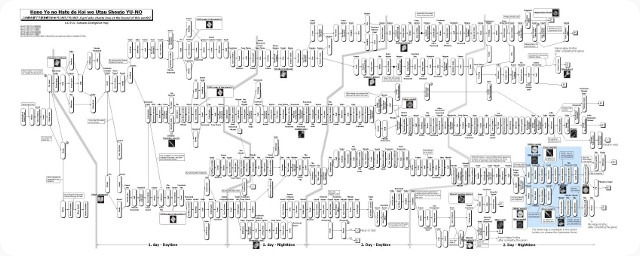
\includegraphics[width=0.9\textwidth]{tree.jpg}
    \caption{Mass Effect storyline graph}
\end{figure}
\vspace{4.0 mm}

As you can see the tree is overly complicated and certain decisions will completely lock-out certain other events from happening. This is an ineffective solution as the player experience is not being optimised. The solution to this problem will be presented later on in the paper.

\vspace{4.0 mm}
\textbf{Online Gaming}
\vspace{4.0 mm}

As mentioned earlier games are increasingly starting to rely on adaptive content to appeal to larger audience. Another example of games using adaptive content is that of online games such as MOBAs (Multiplayer online battle arena) and online FPSs (First-person shooters) which rely heavily on competitive game-play between users from all over the world. Indeed companies such as Valve have even hosted competitions for their game Dota 2 \textsuperscript{TM}, with the prise money reaching 10 million dollars for the winning team in the last such competition. This show that these games are really starting to build traction and as such are starting to earn their respective owners a lot of money.
\vspace{7.0 mm}

Since these games are online they have the very real problem of players harassing each other. Harassment in these games occur for a wide variety of reasons and punishment of problem player does not usually prevent further harassment.  To combat this certain gaming companies have implement machine learning algorithms that monitor all online matches occuring and along with a few questions that each player must answer determine who players are matched up with when they play. These algorithms keep the obvious goal in mind of keeping problem players seperate from players who are well behaved. This tactic has been commonly referred to as the `prison island' tactic by gamers. Another outcome is so that problem players are punished automatically without any other players having to complain.
\vspace{4.0 mm}

\begin{figure}[h!]
    \centering
    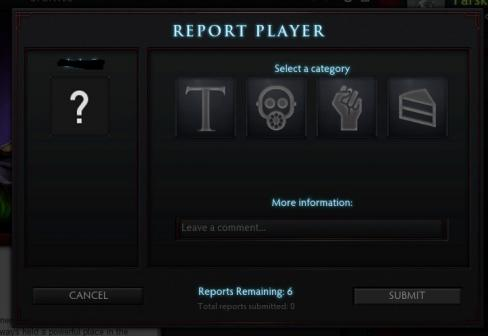
\includegraphics[width=0.5\textwidth]{report.jpg}
    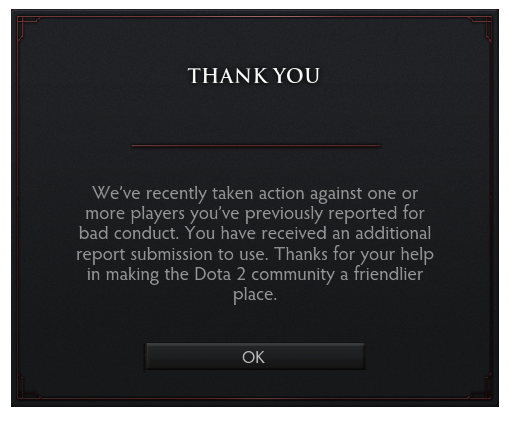
\includegraphics[width=0.5\textwidth]{question.png}
    \caption{Dota 2 report system}
\end{figure}
\vspace{4.0 mm}

Certain games also deploy tactics to team players up with other players who have the same skill level as they do. To do this, these companies monitor players scores and move them up or down in `rankings' appropriately. This is not a perfect system though as scores do not perfectly reflect player ability and has in some cases incorrectly placed players with high skill levels in low skill divisions and vice versa. As these games are competitive, this can create quite a lot of strife within the communities, even forcing players to abandon the games out of frustration losing the gaming company any revenue they could have expected from these players. Better algorithms at placing players in the correct division could thus potentially save these companies a lot of money.


\vspace{6.0 mm}

\subsubsection{Viability of Adaptive Content}

As shown in the introduction the need for this research was justified by saying that more people are using technology on a daily basis but not all of these people are capable of using technology efficiently. How then can this issue be tackled to help these people improve their performance when using computers? It was shown in \citep{beaudry2005understanding} how users of varying technological ability responded to a new technology being introduced in to their work environment. The paper found that although peoples reactions and abilities to adapt vary widely for each individual, it is possible for these adaptation `Strategies' to be grouped. The research concluded by observing actual people in real life scenarios that there are four broad adaptation strategies that cover all individuals coping mechanisms to new technology. This is highly important since it shows that if it is possible to label an individuals coping mechanism and behaviour then it is possible to develop a method to help any individual cope with new technology.

\vspace{6.0 mm}


How though can we implement this? How is it possible to create something that will automatically fit a person to effectively minimise the time they take to cope with new technology? There are several papers that have provided a solution to this problem. They propose that to optimise a users performance, one must simply adapt the interface of said program to perfectly suit the user \citep{lavie2010benefits}. Whether or not this is applicable is another problem, as adaptive interfaces might be to hardware intensive or the creation of different interfaces as opposed to a single broader interface might be cost ineffective.
``Benefits and costs of adaptive user interfaces" by Lavie Talia and Meyer Joachim gives an outline of an experiment where this is explored. Through the use of an experiment involving people of different ages operating vehicles with different interfaces and then measuring their response times,
they came to the conclusion that adaptive interfaces are beneficial in situations where computation time is not an issue. They also came to the conclusion that older peoples' performances improved drastically when using adaptive interfaces but younger people's performance either remained unchanged or dropped drastically. In these cases the interfaces actually impeded user performance.
\vspace{6.0 mm}

This shows that it is possible to create an adaptive interface which can improve user performance but it was noted in Lavie and Meyer \citep{lavie2010benefits} that further research was required to explore and expound upon this topic. 
\vspace{6.0 mm}

\subsection{Markov Decision Processes}

How then can an adaptive user interface be generated? There are several methods to accomplish this. The method that has the lowest apparent computation time and most apparent usefulness makes use of what is called a Markov decision process \citep{sutton1998introduction}. ``Reinforcement learning: An introduction"  \citep{sutton1998introduction} explains in detail the applications of a field of computer science called reinforcement learning. Reinforcement learning is a machine learning process whereby the environment learns from the users interaction with it. The book also covers a very broad range of applications, seeing use in topics such as genetic algorithms, psychology, control engineering etc. However there are several challenges with reinforcement learning. The major challenge is the trade-off between what is referred to as exploitation and exploration. To achieve a high reward, reinforcement learning must exploit as many decisions it has observed in the past. However, to obtain these decisions it must explore as much as possible, which might lead to massive training data. The paper then goes on to explain that there is no easy way to pick an optimal route between exploitation and exploration.
\vspace{6.0 mm}

A Markov decision process is a mathematical framework that can easily represent decision making when some decision may be random. Its most common representation is that of a directed graph where states and actions are nodes and the connections between these are probabilities of certain events occuring. Through the use of an MDP, we can easily create an iterative method that updates states and actions so that an optimal policy is possible. In conclusion the paper shows that reinforcement learning can generate agents  whose performance improves over time through computational effort.\citep{white1991survey}
\vspace{6.0 mm}

These MDPs have been used in \citep{ramamoorthy2013latent} and \citep{rosman2014user} to generate interfaces. The MDPs were represented using the list data structure with look-up times increased using hash tables. In \citep{andrade2005challenge} a representation of a basic MDP is shown. They used a list structure with each state mapping to several actions as well. Using this, the program can measure user's actions and then store them over several 'games'. This data can be averaged to show the behaviour of the user. Knowing which actions have better results will allow us to tweak the user interface so that the user picks better action more often.
\vspace{6.0 mm}

Formally, an MDP can be defined as follows. 
\begin{itemize}
	\item Let S be the set of states in the MDP
	\item Let A be the set of actions in the MDP where A\textit{s} are the set of actions available at state s
	\item Let Pa(s, s') be the probability of an action a being taken at state s to the state s'
	\item Let Ra(s, s') be the reward of taking action a from state s to state s'
\end{itemize}
\vspace{6.0 mm}

\begin{figure}[h!]
    \centering
    \includegraphics[width=0.3\textwidth]{MDP.jpg}
    \caption{Basic Representation of an MDP}
\end{figure}
\vspace{6.0 mm}

\begin{figure}[h!]
    \centering
    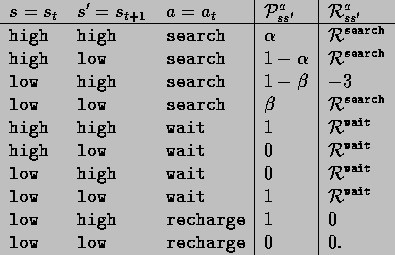
\includegraphics[width=0.6\textwidth]{1.jpg}
	\caption{Example table}
\end{figure}

\begin{figure}[h!]
	\centering
    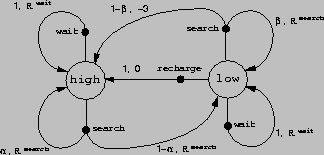
\includegraphics[width=0.6\textwidth]{2.jpg}
	\caption{Corresponding graph}
\end{figure}
\vspace{6.0 mm}
\FloatBarrier

\clearpage

So it has now been shown that adaptive interfaces can indeed be made and that through the use of an MDP we can generate a user profile for each user. All that needs to be shown is how to actually create and decide on interfaces for users. The method for doing this quite clear cut \citep{dessart2011showing}. All that must be done to adapt the interface is to create a transition function which is done as follows:
\begin{itemize}
\item Find what action has been changed by the user.
\item Find which element of the user interface is affected
\item Perform one of the following operations on the element: Resize, Relocate, Image transformation, Widget transformation, Widget splitting.
\end{itemize}
\vspace{6.0 mm}

There is one more thing that needs to be shown. Once a user profile is selected and an appropriate interface selected, the user is then given the newer interface to use. After this the program will hone in on an optimal interface until the user is always performing his/her optimal actions \citep{dessart2011showing} \citep{andrade2005challenge}.

\vspace{6.0 mm}

An adaptive interface isn't exactly easy to implement due to computation constraints. Further study can be done in creating adaptive interface algorithms more efficiently. A computer game usually requires a large amount of computation power. This has large implications for the tech industry since several devices require a calibration stage before usage. An adaptive interface can be used to circumnavigate this and instead perform the 'calibration' on the fly. Take for example the computer game system called the xbox. Users upon first starting the console up must perform several basic adjustments to alter the interface to suit themselves. Most users find this highly annoying and often write complaints on this very issue to manufacturers as a result.
\vspace{6.0 mm}

\clearpage

\subsection{Conclusion}

Overall, this research has never been fully explored and has only been implemented a few times in small contained experiments such as those in \citep{andrade2005challenge}, \citep{ramamoorthy2013latent} and \citep{rosman2014user}. Adaptive content has been implemented in computer games but not to the large extent that is being proposed with the use of MDPs. Since this approach does not simply have to be used in the generation of user interface but can be used to map user preferences and behaviours. Due to this fact, there is a lot of room for improvement and exploration. Thought has been given to use this approach in the generation of RSS feeds on the internet. Even advertisements can use this method to create user profiles and then a mapping from one advert to another. This research can, quite literally, be used in almost every aspect of computer systems since most computer systems are used by people with varying skill levels and understanding of computers. This research will explore and tackle this in a way that can be implemented anywhere.
\vspace{6.0 mm}

Therefore it has been proposed that an interface can be created which will increase the users performance. Which can be summarised as follows:
 The content and interface of a computer program can be updated or changed to automatically improve the users performance.
\\
The commercial and societal impact of this research has been shown to have merit by showing that several companies would benefit directly from this research. Lack of research in this area of computer science indicates that more research is required to further this field. Many new and novel ways have also been suggested to generate adaptive interfaces but have not been fully explored.



\clearpage
\section{Research Method}
\subsection{Introduction}
The research being discussed in this section has two primary goals. Firstly the research aims to verify that adaptive content in computer games improves the users' performances. Namely research done by Subramanian Ramamoorthy, MM Hassan Mahmud, Pushmeet Kohli and Benjamin Rosman \citep{rosman2014user}, \citep{ramamoorthy2013latent}. Secondly it aims to implement and expound upon the method provided in these papers in a more complicated gaming environment. This chapter provides the basis by which the research aims to achieve this.
\vspace{6.0 mm}
\subsection{Motivation and Hypothesis}

Rosman and Ramamoorthy \citep{rosman2014user} have shown that it is possible to create an interface which is better suited to the user. Even though this interface might actually initially impair performance, Rosman and Ramamoorthy have shown that the users will reach a higher performance with the newer interface over time. In addition it was shown that the time taken for the user to adapt to the new interface will decrease if intermediate interfaces are provided to the user. Where intermediate interfaces are interfaces that incrementally add changes to the existing interfaces such that the user is not overwhelmed by the new changes. Previous research thus allows us to make three assumptions that we will base our work on:\\
\begin{itemize}
\item Skill level can be quantified
\item Skill level can be inferred from user behaviour
\item Aspects of the game can be adjusted to affect the user experience
\end{itemize}

\vspace{6.0 mm}

In all other research, experiments were done with relatively simple games (such as navigating mazes). In these experiments the actions the player made could be very easily linked to a change in the MDP. However, if this idea is to be implemented in other real-world scenarios, the changes in the MDP might not be as obvious. Take for example a game where a player could pick from 100 possible actions as opposed 4. The representation of the MDP we are familiar with would not be helpful in this scenario and it would be difficult for us to visualise such a MDP. Therefore, we our research aims to contribute to this existing research by focusing on a more complex game, where there might not be an optimal choice to be made.
\vspace{6.0 mm}

Which comes to my research hypotheses (Note that these both apply to complex games):

\vspace{6.0 mm}

\begin{flushleft}
\textbf{
Hypothesis 0:} \centering{The content and interface of a computer program can be updated or changed automatically based on skill level.}

\vspace{4.0 mm}

\textbf{
Hypothesis 1:} \centering{Adaptive content improves the users' experience.}
\end{flushleft}

\vspace{6.0 mm}

\subsection{Overview of Method}
\subsubsection{Programming Languages}
All programming done in performing this research will be done in python using the PyGame and NumPy libraries. MDPs will be represented as a linked list. The reasons are as follows:
\begin{itemize}
\item Python is relatively simple to use
\item We have experience in using Python as well as the similar language Java
\item Python has several useful libraries
\end{itemize}
\subsubsection{Phase 1: Game Design}
Although we aim to extend the game to more complex games, this does not necessarily mean we should become over-ambitious in our game choice. Thus a game must be chosen that has several choices available to the user at each stage, but not too many choices, as we want to be able to finish the research within the current time constraints.
\vspace{6.0 mm}

Taking all of this into account, we have decided on implemented a simple `Tower Defence' game. The reasoning in this decision is as follows. Tower defence games are a classic sub-genre of strategy games, having been seen in gaming in its infancy as far back as 1990. It has remained a popular genre till today with most `gamers' having at some point played a variation of tower defence. This popularity and familiarity with the genre will aid in testing as it will be easy to round up testers who are skilled.
\vspace{3.0 mm}
The `gameworld' in tower defence looks as follows:


\begin{center}
    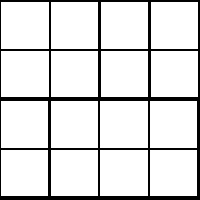
\includegraphics[width=0.2\textwidth]{grid.jpg}
\end{center}




This basic grid layout will help keep programming the game simple. The goal of tower defence games is to prevent enemies from reaching some point on the grid. Enemies start at some point in the grid then proceed to follow some predetermined path on the grid.


\begin{center}
    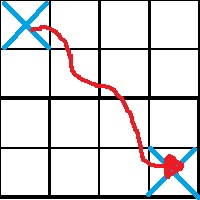
\includegraphics[width=0.2\textwidth]{path.jpg}
\end{center}


To accomplish this towers are place by the user at any point on the grid besides the point that are `paved' for the enemy. Each placed tower will fire upon nearby enemies. However, the player must take economy into account as each tower costs in-game money to build and each enemy destroyed provides the player with this money. Enemies also appear in `waves' such that the gameplay is staggered giving the player time to think and place towers.
\vspace{3.0 mm}

\begin{figure}[h!]
    \centering
    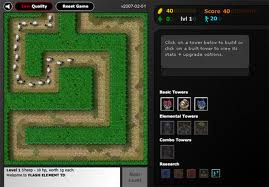
\includegraphics[width=0.6\textwidth]{td1.jpg}
    \caption{Popular Tower Defence Warcraft 3 mod}
\end{figure}
    \vspace{1.0 mm}
\begin{figure}[h!]
    \centering
    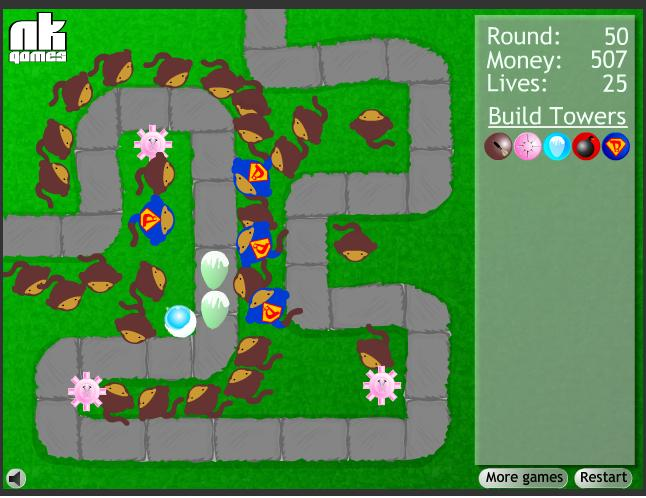
\includegraphics[width=0.6\textwidth]{td2.jpg}
    \caption{Popular iPad Tower Defence game}
\end{figure}

\vspace{3.0 mm}

On top of all this there are usually different types of enemies and towers which further increases the amount of decisions that the player can make at each stage. This complexity gives us manoeuvring room as there are several options to pick from that could help us alter the games difficulty. For example, if we see the player is struggling to cope and is letting more and more enemies through their defence then we could perhaps alter the game by decreasing the amount of enemies, making enemies easier to defeat, removing the type of enemy the play is struggling with, changing the cost of towers etc. This wide range of options makes the experiment easier to conduct by giving us more information to work with. The programming of this game should not take too long to accomplish but the games parameters and design will change constantly throughout all other phases of the research. This is purely due to the fact that certain variables may be discovered to yield better results.
\vspace{3.0 mm}


\subsubsection{Phase 2: Testing}

The second phase of the experiment will require testing to be done on players of varying skill levels. The testing will require players who are familiar with tower defence games, people who are familiar with computer games in general and people who are not familiar with computer games in general. These groups of players will correspond to skilled, intermediate and unskilled levels respectively. They will then be required to complete the game. Certain variables will be recorded and then used to determine each users play style respectively. Players will also be required to rate the games enjoyability.
\vspace{6.0 mm}

All independent variables available will be recorded. Giving us as much information as possible to connect player levels to MDPs. For example, when a player places a tower, the stage at which he placed the tower, its position and the towers type will all be recorded. This would tell us what actions each type of player would make given possible options. However, the most informative variables and the unimportant variables will not be obvious at this point so as much data as possible must be collected. After all the data is collated and sorted, we can then move onto the algorithm design phase.
\vspace{6.0 mm}

\subsubsection{Phase 3: Algorithm Design}

After all the data is collected regarding each players `play style' we now have information with which to create our MDPs. Where the state of the game is the current wave number and the action is the tower placement. The following definition are required:
\vspace{6.0 mm}

\begin{itemize}
	\item Let S be the set of states in the MDP
	\item Let A be the set of actions in the MDP where A\textit{s} are the set of actions available at state s
	\item Let Pa(s, s') be the probability of an action a being taken at state s to the state s'
	\item Let Ra(s, s') be the reward of taking action a from state s to state s'
	\item Let M be the set of all MDPs
	\item B is the updated MDP
	\item N represents the function by which B is being updated in algorithm 1. N is usually a Q learning algorithm.
	\item  
	\begin{equation}
	B' =  argmax{|B| \sum f(s1:k, Y) > |B| - 1 + \beta}
	\end{equation}
	
\end{itemize}

\clearpage

\begin{lstlisting}[label=Algorithm,caption=Algorithm 1: MDP update]
	Initialize all variables
	B(0) = S(k)
	t = 0
	while true do
		Learner choose action A(t)
		Learner obtains some reward R(A(t))
		Nature returns set B(t+1) = N(A(t),B(t),T)
		t = t + 1
	end
end
\end{lstlisting}
\begin{lstlisting}[label=Algorithm,caption=Algorithm 2: Online Interact]
	Input is the set of all MDPs M and X the selection policy
	As well as the constant beta, f and term where beta is a constant
	term is the task termination condition
	Initialize all variables
	B(0) = S(k)
	Let Y be the uniform set over S for each a and s
	Set all r to be 0 for each a and s
	t = 1
	while term =false do
		Get a, r and s at t
		Get all possible s and r after taking action a at state s and call these s1:k and r1:k
		Compute B'
		B(t+1) = B(t) - B'
		if B(t+1) is empty then
			B(t+1) = S(k)
		Set A(t+1) = X(B(t+1))
		t = t + 1
	end
end
	
\end{lstlisting}

\vspace{6.0 mm}
\subsubsection{Phase 4: Comparative Analysis}

Similarly to phase 2, the game with the machine learning algorithm now applied, will be presented to skilled, intermediate and unskilled players. Their performances are then recorded as before with all in-game variables necessary such as tower position and type as well as wave number. A direct comparison will then be done between their performances and those of the players in phase 2 to map the performance change in each group. Appropriate graphs and other visual aids can then be created to aid in this comparison. This phase will allow us to decide on the best and most optimal MDPs. Players will also be asked to rate the enjoyability of the game as before in the no adaptive version. These two results will be taken into account to determine whether or not players prefer the normal game are the version with the adaptive content.
\vspace{6.0 mm}
\clearpage
\subsubsection{Time Management}
Taking all of these tasks into account and by estimating how much time we expect to use in accomplishing these, we have created a schedule.
\vspace{6.0 mm}

\textbf{Timeplan:}
\begin{center}
	\begin{tabular}{ | p{6cm} | p{2cm} | p{2cm} | p{2cm} | p{2cm} |}
		\hline
		Task: & Time:       & Start:   & End: & Progress: \\ \hline 
		Finish Research Proposal & 1 Week & 7/3/2014 & 7/13/2014 & Complete  \\ \hline 
		Program Game & 2 Weeks & 7/13/2014 & 7/27/2014 & Underway  \\ \hline 
		Test users for each skill level and collect data & 1 Week & 7/27/2014 & 8/4/2014 & Underway  \\ \hline 
		Create Markov Decision Process for each skill level
 & 3 Weeks & 8/4/2014 & 8/25/2014 & Incomplete  \\ \hline 
		Finish algorithm to map transitions
& 2 Weeks & 8/25/2014 & 9/9/2014 & Incomplete  \\ \hline 
		Test adaptive algorithm on each group and collect data
 & 1 Week & 9/9/2014 & 9/16/2014 & Incomplete  \\ \hline 
		Analyse and compare results to determine viability
 & 3 Weeks & 9/16/2014 & 10/17/2014 & Incomplete \\ \hline 
 Complete research document
 & 2 Weeks & 10/18/2014 & 10/30/2014 & Incomplete \\ \hline 
	\end{tabular}
\end{center}
\vspace{6.0 mm}

\subsection{Conclusion}
The aim of this research is to provide empirical data to verify adaptive content as a viable option in computing. The method for accomplishing these goals was laid out in this chapter with supporting motivation and hypotheses. The method was broken up into 4 phases, two of which were development phases and two of which were testing phases. The method was taken from Rosman and Ramamoorthy \citep{ramamoorthy2013latent} and then improved upon to fit a more complex scenario. The algorithm to do so was provided. The time that we expect all of these tasks to be done in was provided as well. The next chapter will describe what results we hope to gain from conducting this research.


\vspace{6.0 mm}
\clearpage
\section{Results}
\subsection{Introduction}

It is necessary to explain exactly what results we expect to obtain from our research are. In this section we will explain what results we expect to see and exactly what we hope to achieve with this. As well as explaining how unexpected results would affect our research. The consequences of our research will also be discussed. Due to the nature of this section, an overview of what future research could be conducted.

\vspace{6.0 mm}
\subsection{Expected Results}

It is quite clear that the experiments must show that user performance and scores increase when using the adaptive content algorithm to play the game. We expect players report the game as being more enjoyable. In the event results are not what we expect then we will tweak and modify the game to determine if the problem arose there or with the algorithm itself. In the unlikely event neither of these options are true then we can safely say that our entire experiment is flawed. The implications of the expected results would mean that this algorithm could be then implemented in several real world systems to improve their usability.
\vspace{6.0 mm}
\subsection{Future Work}
This algorithm can be implemented in real world scenarios as well as being modified to perform better. As shown earlier in the literature review, I described examples of real world instances of content adaptation. In the first example I showed that computer games create alternate storylines in their games usually represented as a complicated graph. With the use of this algorithm, this entire structure can be scrapped and the developers can create entirely unlinked quests. This pool of story points or quests can then be drawn from by the algorithm to best suit the individual user. The developers will now be able to structure the quest system of the game in a way that can keep each player optimal. There are additional side-effects though, each player could possibly have a unique experience which will keep player replaying and immersed in the game. Developers can now add content to the game in small updates rather than developing massive expansions by simple designing single quests that can be added to the list of quests the algorithm can pick from.
\vspace{6.0 mm}

In competitive games, the algorithm could be applied to better keep players of similar skill-levels playing together. Which could potentially reduce frustration amongst the community and thus keeping the amount of moderation by the company down to a minimum. Work could also be done in testing the algorithm for other scenarios than gaming. As in most sciences, there is always room for improvement, research could be done into developing a more sophisticated algorithm that has lower computation times and more accuracy. It might be possible to refine the algorithm so that it consumes less system resources such as memory. As shown previously by Krzystof Z Gajos, Jacob O Wobbrock and Daniel S Weld \citep{gajos2008improving}, adaptive interfaces may require too much computing power for them to be useful in real-life/ real-time scenarios. Thus much work can be done into improving this algorithm.
\clearpage
\section{Conclusion}
The viability of this research was conducted by several scientists using several different experiments to show that it is indeed possible and useful. Rosman and Ramamoorthy \citep{rosman2014user} developed an algorithm that could be implemented to alter the interface of the game to improve user performance. Their research showed that such an adaptive interface did improve the users experiences with the aid of staggered transition interfaces to ease the user into the new interface. The algorithm to do so was presented in their papers. It was determined that it was necessary for further research to be conducted to explore this algorithms use in more complex scenarios. This research aims to expand on this algorithm by implementing it in a more complex scenario.
This proposal provided a groundwork for creating this algorithm. It also provided a literature review that effectively explains the process by which we have reached this idea as possible research. 
\vspace{6.0 mm}
Future work can be done into refining this method into a more robust method. That can be implemented quickly and effectively into other situations. Situations such as basic software and perhaps web-development could see use of this algorithm in their implementation. Existing game developers could make use of it on a broader scale by incorporating it into existing games titles. Altogether, the algorithm has a wide range of uses in computing and could possibly reach many markets. As such, all these factors contribute to us thinking of it as a highly sophisticated approach to the way developers present content to their users and as such we see it as a viable research topic.

\clearpage
\bibliography{references}


\end{document}
